\chapter{Experimental methods}
\label{ch:Experimental setup and methods}
This chapter presents the experimental setups and methods applied to characterise of the FBK and Hamamatsu detectors.

%
% Section: ======================
%
\section{IV curve}
\label{section:IV curve}
The IV characteristic curve represents the measured current of the detector as a function of the bias voltage and can be used to calculate $V_{bd}$ and $R_Q$. Due to the temperature dependency of the quenching resistor, the measurements are performed at constant temperature. This condition in maintained by the activation of an air conditioner in the laboratory. 
Measurements are taken in the light to reduce the signal to noise ratio. 
\subsection{Breakdown voltage} 
The breakdown voltage $V_{bd}$ can be obtained by studying the reverse biased region of the IV curve (where the current shows a steep increase). Several fitting methods to determine $V_{bd}$ where tested
%as explained in \cite{} 
but preliminary results where not as accurate as the method presented in \ref{ch:Experimental methods:breakdown voltage}. 

\subsection{Quenching resistor} 
\label{ch:experiement methods:IV:Rq IV}
The quenching resistance is a key property of a SiPM. In order to measure it, the IV characteristic curve is obtained in the Forward bias operating mode. In this region, the non-linearity of the diode is overcame by the linearity of the quenching resistors ($R_Q$) making the current response proportional to the bias voltage. The slope of this response is used to compute $R_Q$.
The measurement setup is shown in Fig. \ref{fig:pic IV rq setup}. One channel of the SiPM array is connected to a KEITHLEY INSTRUMENTS 2400 source-measure unit with a \SI{50}{\ohm} resistor in series. To avoid any other internal resistors in the electrical circuit, no other apparatus are plugged. 
\begin{figure}[htbp]
    \centering
    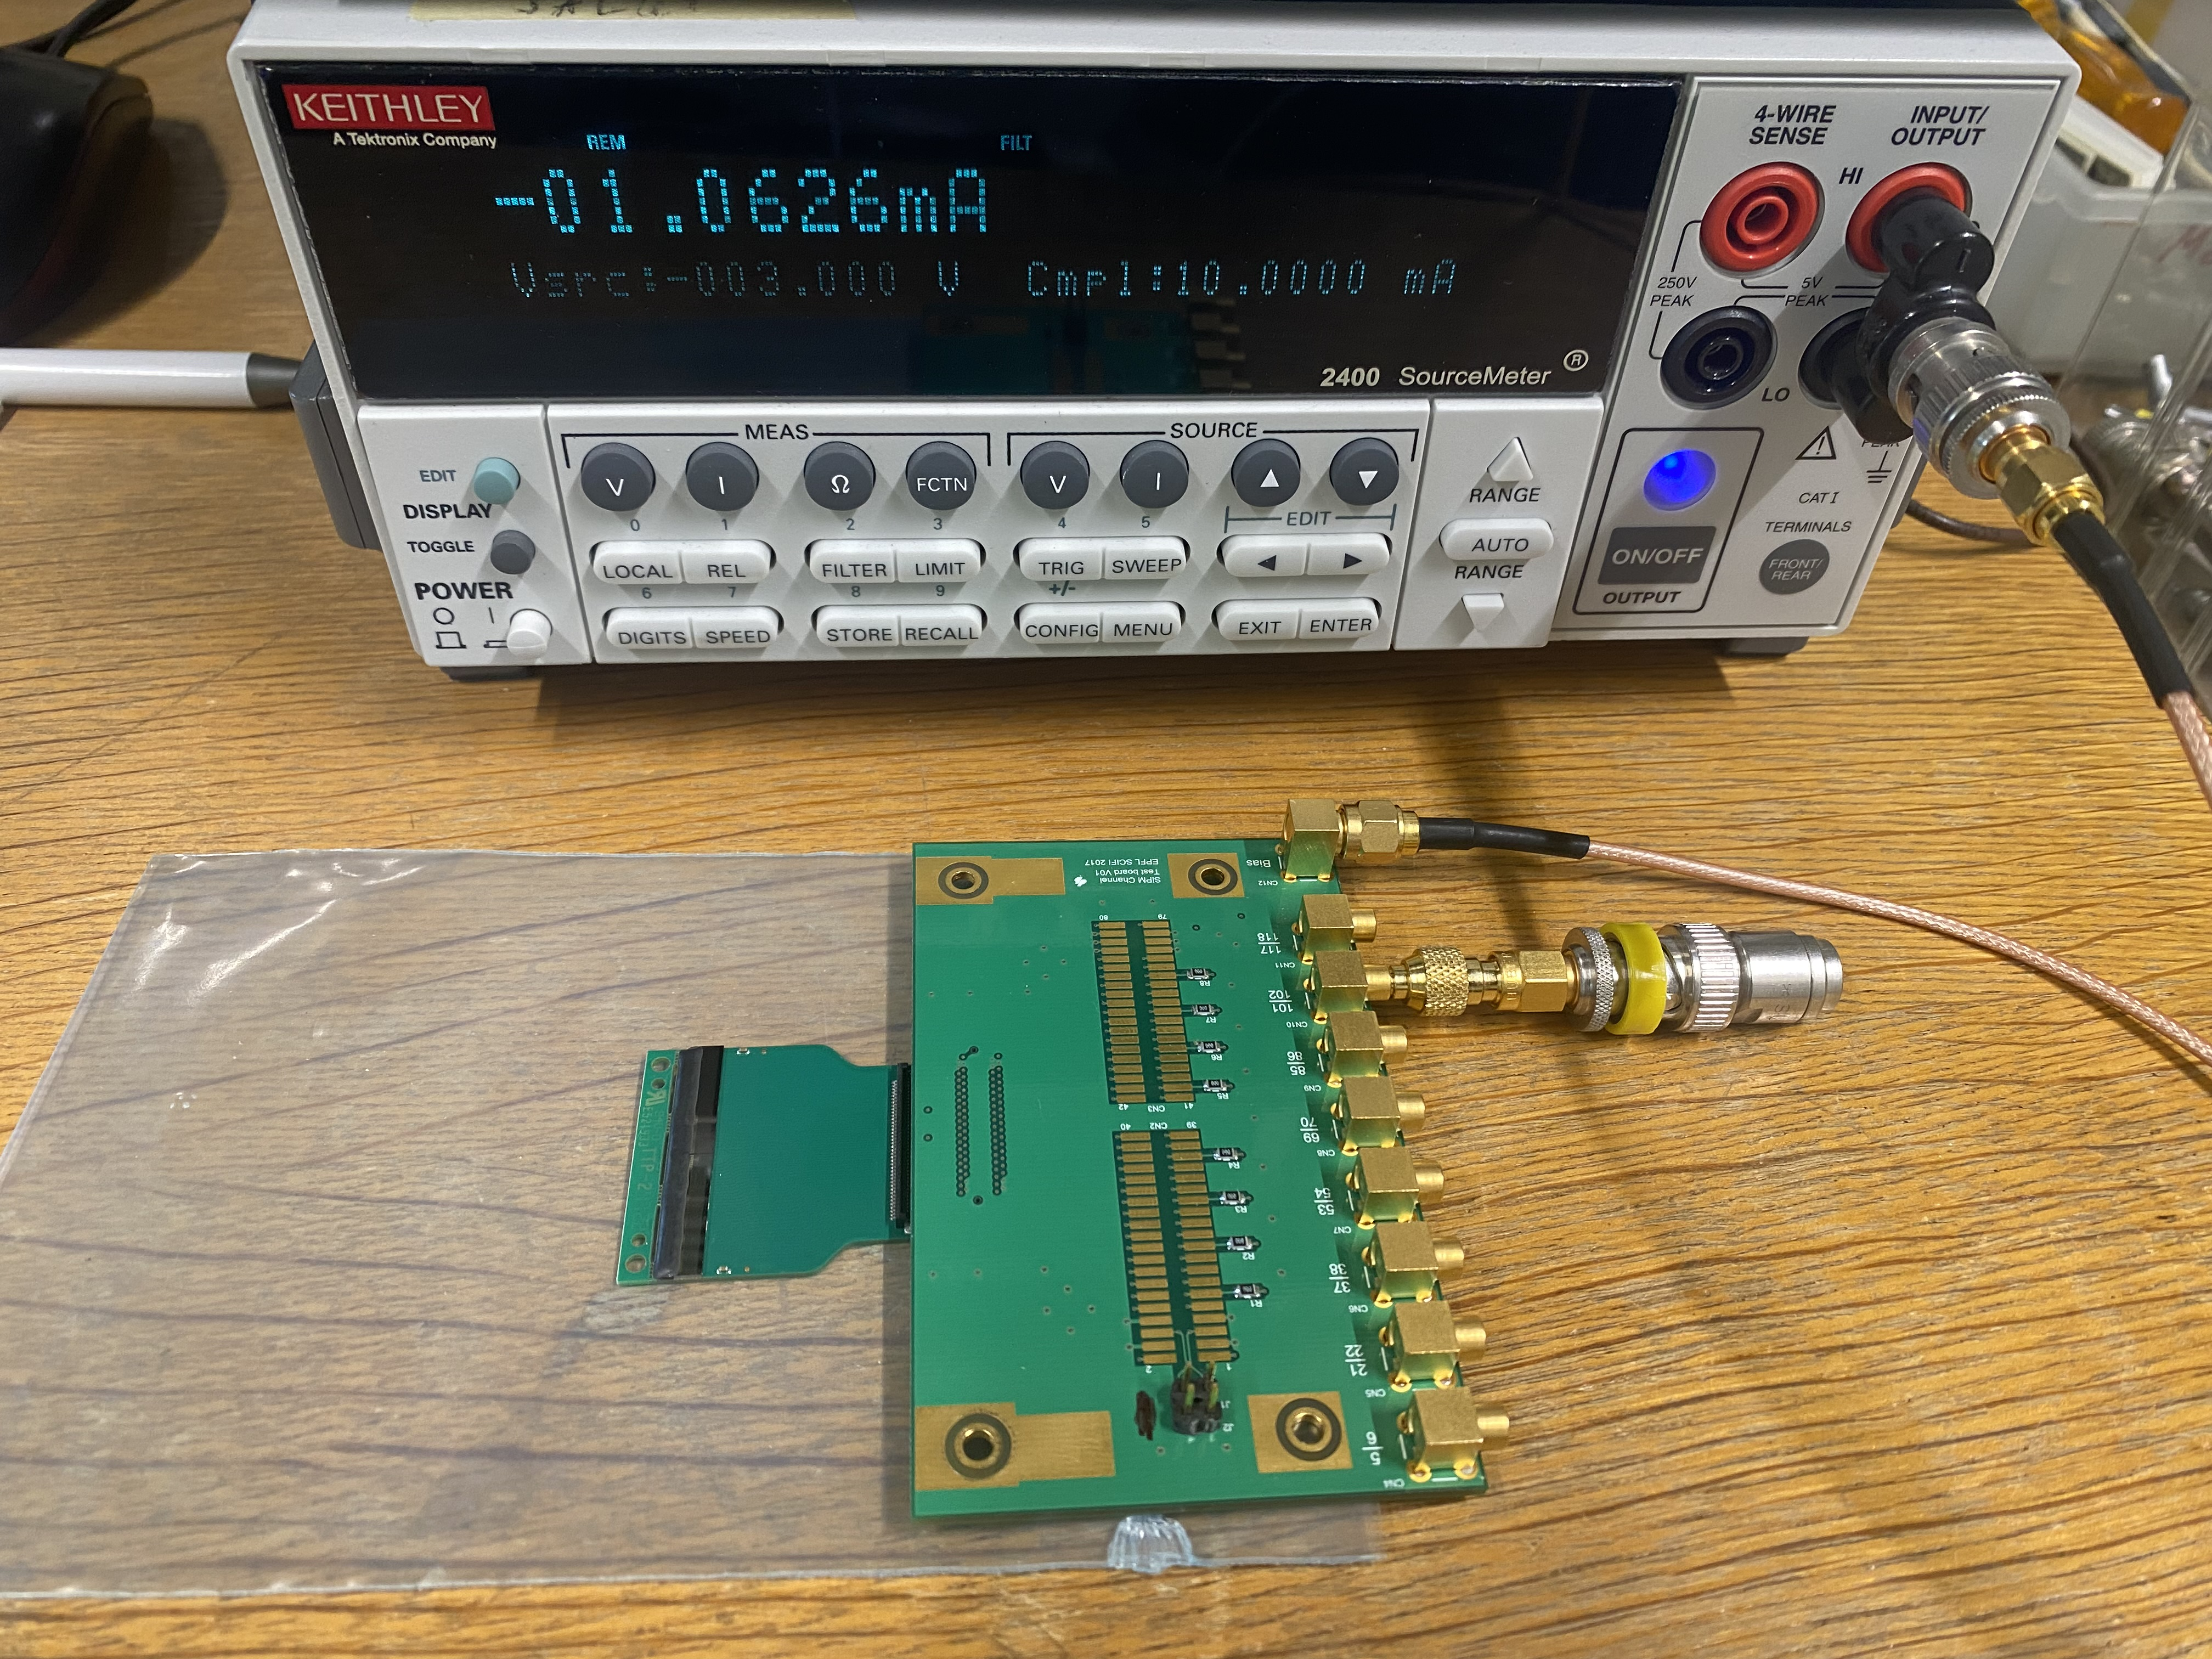
\includegraphics[width=0.8\textwidth]{gfx/pictures/Rq_IV_setup.png}
    \caption{Picture of the experimental setup for the measurement of $R_Q$ with the IV-curve method.}
    \label{fig:pic IV rq setup}
\end{figure}
The SiPM array is connected to a \ac{PCB} where only 8 outputs are available. Theses PCBs allow to characterize 16 channels, 8 ODD and 8 EVEN \footnote{channels analysed: $[5,6, 21,22, 37,38, 53,54, 69,70, 85,85, 101, 102, 117, 118]$}, and minimize the serial resistances from electrical wires. The photo-current coming from the SiPM is measured at different bias voltages in the forward bias region. 
A python script performs the measurement by taking the data from the instrument. An averaging of $10$ current values is taken to counter the influence of noise. 
With this method, the IV characteristics is obtained. The quenching resistance is inversely proportional to the slope of the linear region in the IV curve. In absence of external resistors,  Eq. \eqref{eq:original quenching resistor1} applies:
\begin{equation*}
  \begin{minipage}[t]{0.48\linewidth}
        \begin{equation}
            R_Q = N_{pixels}\cdot \left(\frac{dV}{dI}\right)
        \label{eq:original quenching resistor1}
        \end{equation}
  \end{minipage}
  \hfill
  \begin{minipage}[t]{0.48\linewidth}
        \begin{equation}
            R_Q = N_{pixels}\cdot \left(\frac{dV}{dI} - \SI{50}{\ohm} \right)
        \label{eq:original quenching resistor}
        \end{equation}
  \end{minipage}  
\end{equation*}

Taking into account the resistor of \SI{50}{\ohm} plugged in series to the circuit, the formula becomes Eq. \eqref{eq:original quenching resistor}.
Note that $N_{pixels}$ is the number of pixels contained in one channel for a detector. 
\\
This method is strongly dependent on the choice of the fitting range. Going too high in $V_{bias}$ heats the detectors and changes the value of $R_Q$. On the other hand going too low, the IV curve's behavior is not linear anymore (diode response not negligible). The fitting range has been discussed with the manufacturer to have consistency in the methods \cite{StefanoMerzi2023PrivateCommunication}. For the H2017, the fitting range is the same as in \cite{Girard2018CharacterisationDistributions}. Results are shown in Section \ref{ch:Results:Rq}.

\paragraph{uncertainties.} The statistical uncertainties are negligible due to the goodness of the linear fit. 
Channel to channel, a variation of $5\%$ in the quenching resistor values is observed. The connection between the channel to the IV setup introduce serial resistances order of magnitude of \SI{1}{\ohm}. This error is bigger on the \SI{16}{\micro m} since it has the larger number of pixel $\approx 1\%$ whereas $0.1\%$ for the \SI{31}{\micro m}. The total uncertainties is then $\pm 6\%$ for the \SI{16}{\micro m} and $\pm 5\%$ for the other detectors. 
The results are presented in section \ref{ch:Results:Rq}.


\section{Waveform analysis}
\label{section:waveform analysis}

\begin{figure}[http]
    \centering
    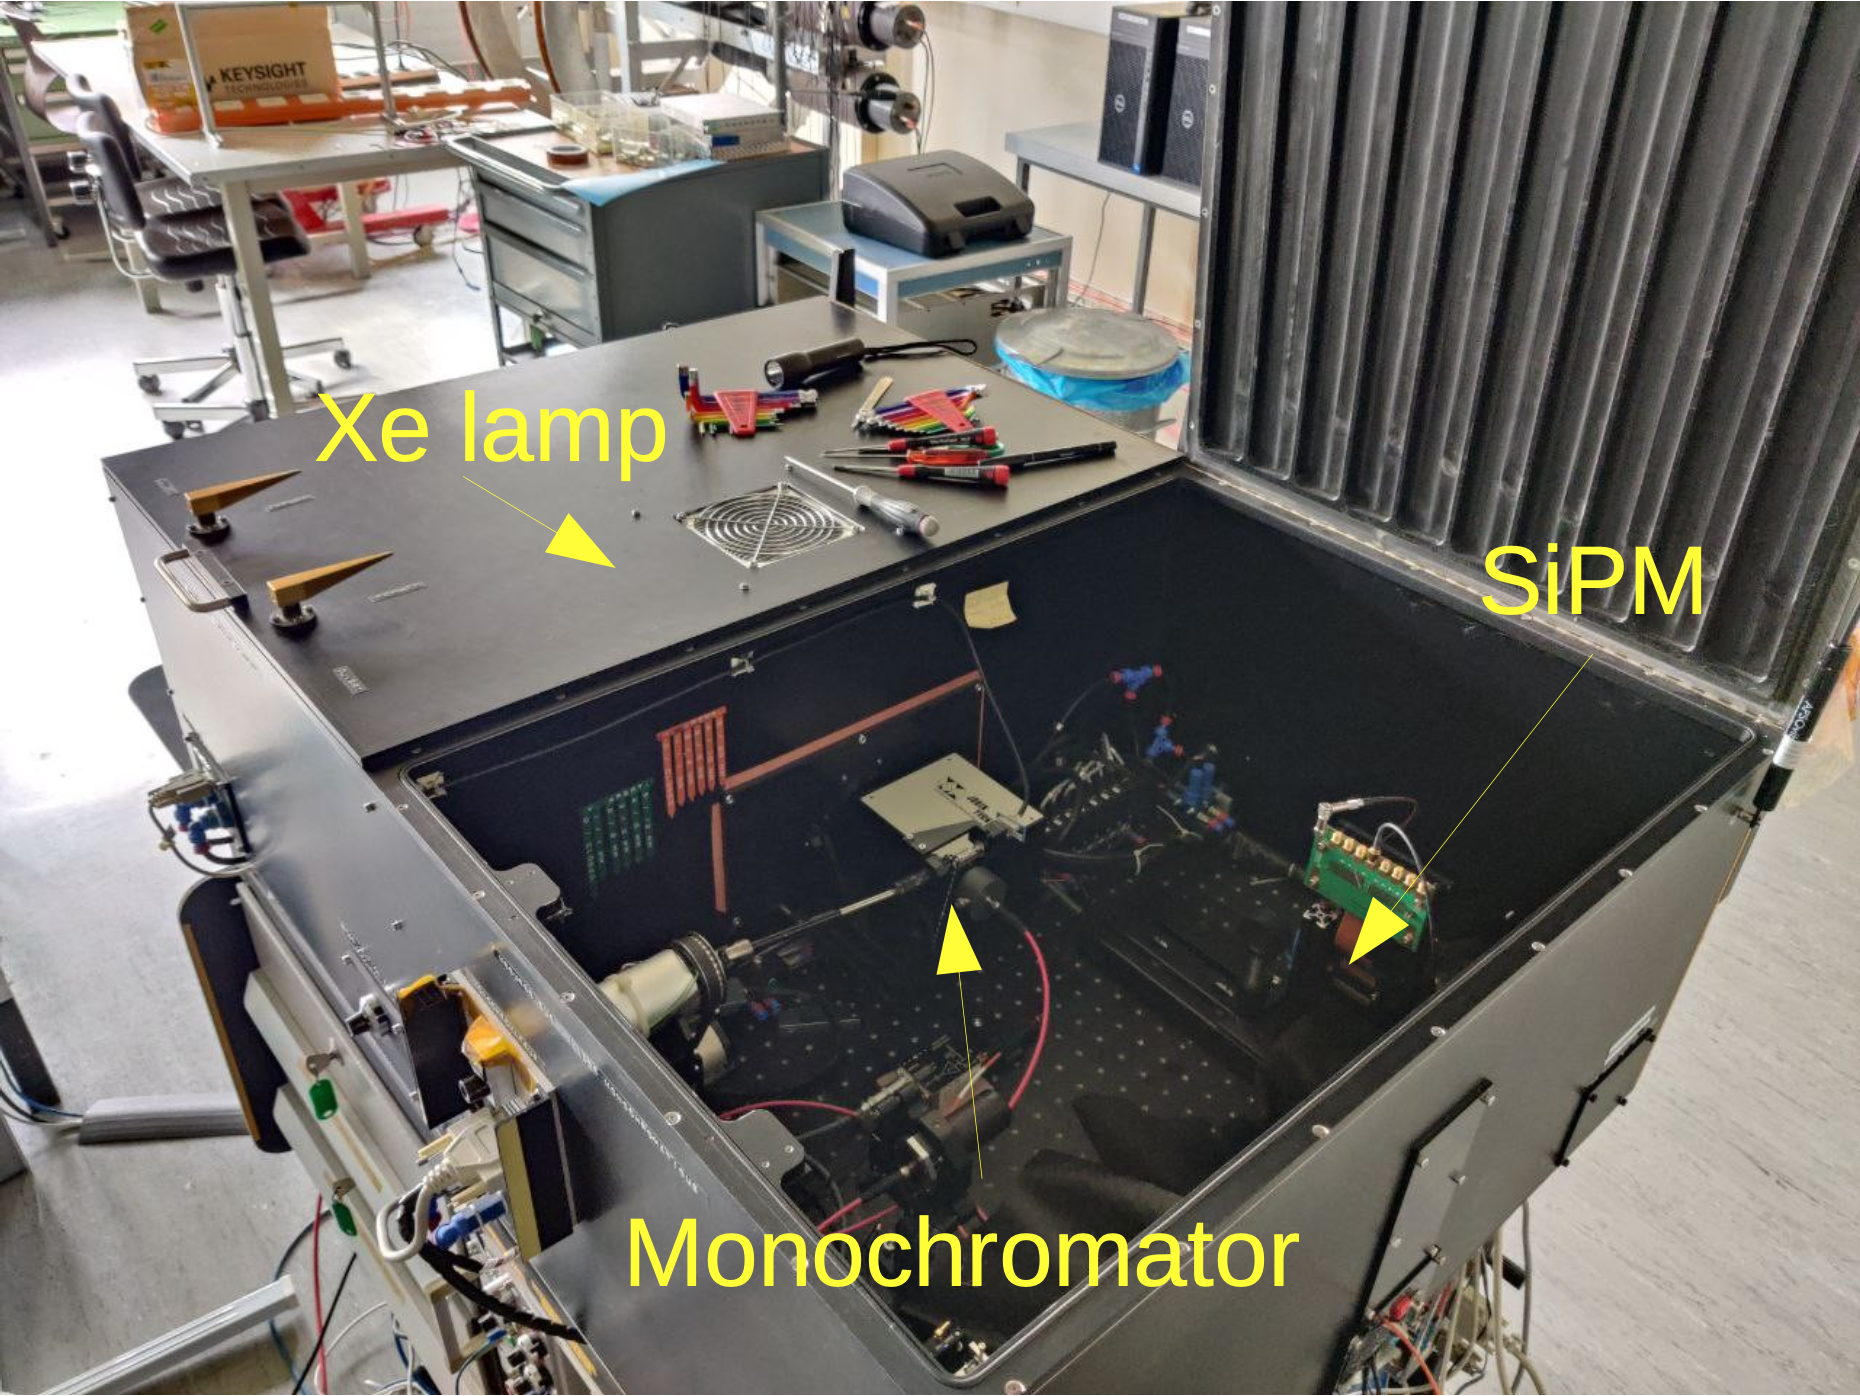
\includegraphics[width=0.8\textwidth]{gfx/pictures/PDE_setup.png}
    \caption{Photograph of the waveform analysis and PDE measurement setup.}
    \label{fig:PDE setup pic}
\end{figure}
Recording the waveforms produced by the detectors allow to measure several characteristics. 
\subsection{Setup}
\label{ch:Experimental setup:WA:setup}
The detector is in a black box shown in Fig. \ref{fig:PDE setup pic} that shields electromagnetic interference to limit the electronic noise\footnote{The Xe light is not used yet (see \ref{ch:Experimental methods:Gain and PDE:setup})}. The detector is mounted on a PCB, connected to a bias voltage\footnote{KEITHLEY INSTRUMENTS 2400},the signal is amplified (\SI{40}{dB}) and connected to the oscilloscope. A picture showing the connection of the channel to the PCB is shown in Fig. \ref{fig:PCB channel picture}:
\begin{figure}[htbp]
    \centering
    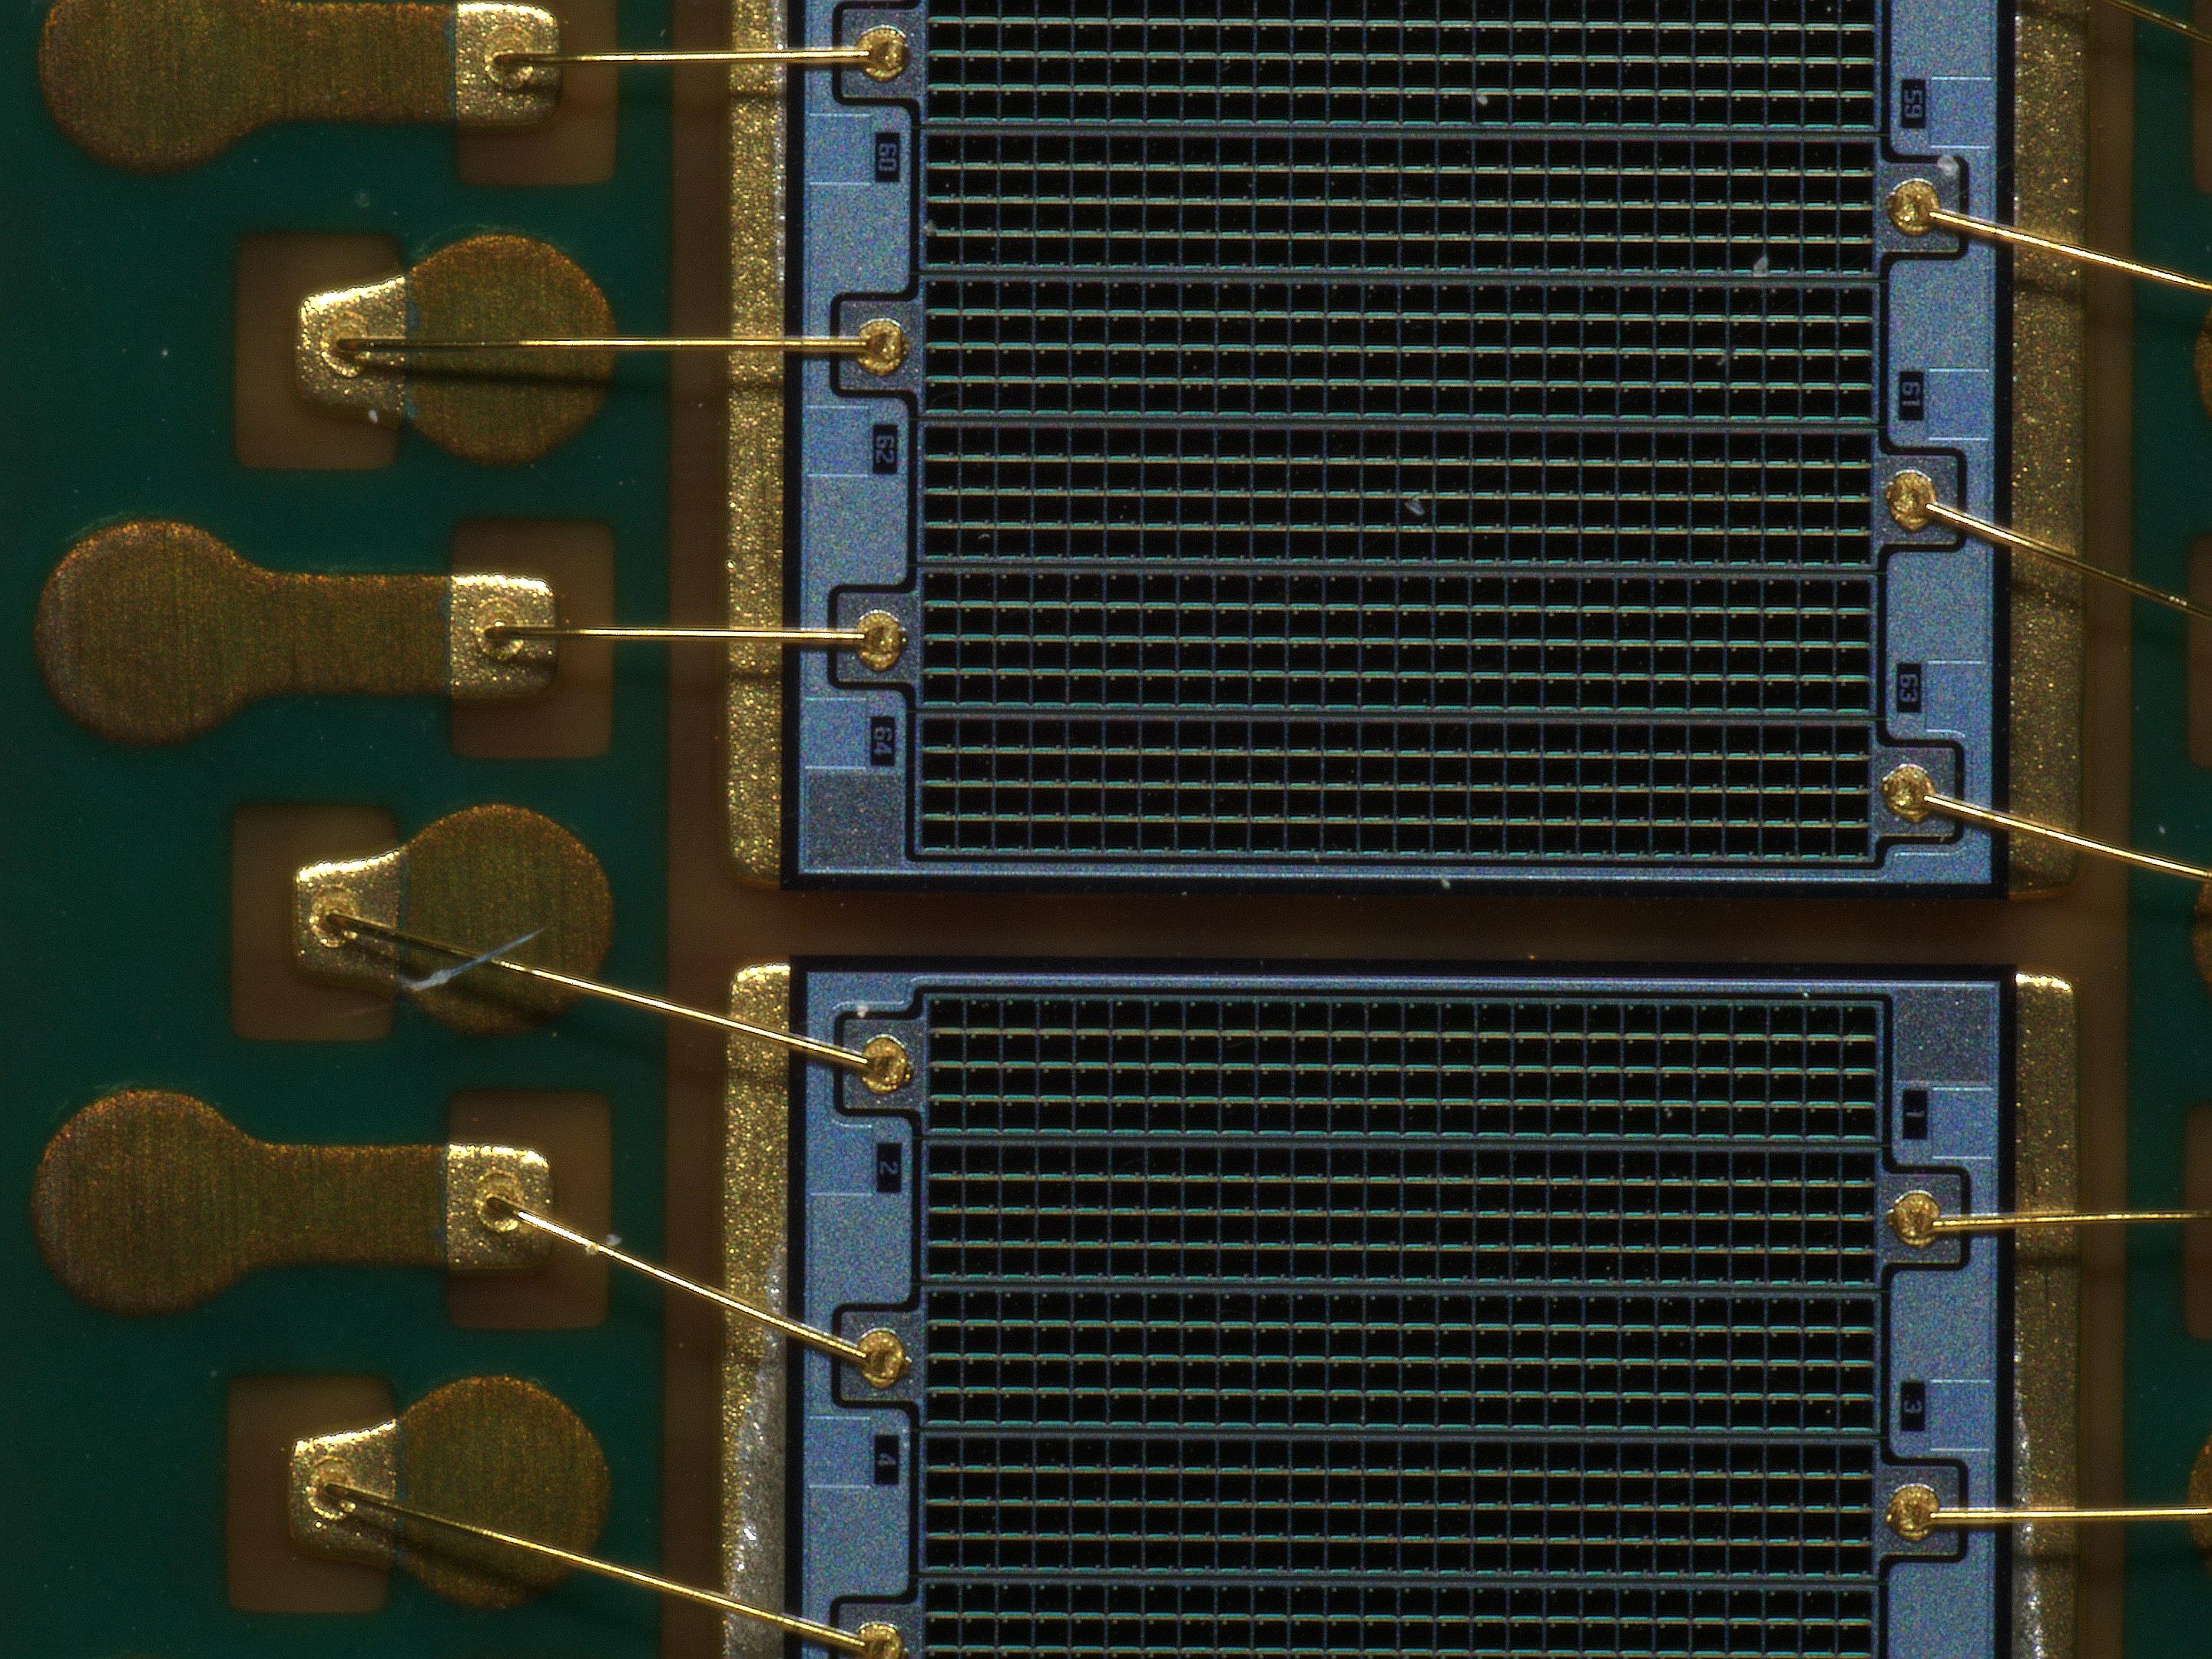
\includegraphics[width=0.8\textwidth]{gfx/pictures/PCBchannel.jpg}
    \caption{H2017 channel bonding to the PCB. Picture taken by G. Haefeli with a Keyence microscope. }
    \label{fig:PCB channel picture}
\end{figure}
A black cloth is wrapped around the detector so that only waveforms corresponding to noise are recorded.
The oscilloscope records the waveforms triggered on a $1$ PE signal, meaning on a dark count. The single photons waveforms are defined as clean waveforms. By doing this, the correlated noise such as DiXT, DeXT and AP are identified on the waveforms with a software. It is important to tune the thresholds for different types of noise, so that the script identifies and classify the waveforms accordingly. The breakdown voltage $V_{bd}$ is also measured by recording the waveforms in this configuration. The measurement are taken at fixed temperature of \SI{25.0}{\celsius} to avoid the temperature dependency of $V_{bd}$ and the correlated noise. A PT100 temperature sensor is connected to the PCB to know the temperatures during the measurement. 

\subsection{Breakdown Voltage}
\label{ch:Experimental methods:breakdown voltage}
By measuring the mean peak amplitude of $1$ PE pulses, such as the one shown in Fig. \ref{fig:mean pulse amplitude}, the breakdown voltage is obtained. 
The relation between the pulse amplitude and overvoltage is linear, therefore the dependency can be fitted and the extrapolation to zero is the breakdown voltage. This method has proven to be really effective and trust full, allowing to reach a level of precision by the order or \SI{200}{\milli V}.


\paragraph{uncertainties.}  The systematic uncertainties are estimated\footnote{Evaluated with different measurements, with different $V_{bias}$ ranges.} to be $\pm$ \SI{200}{\milli V}. Due its lower signal to noise ratio, the systematics uncertainties as expected to be higher for the FBK \SI{16}{\micro m} with $\pm$ \SI{300}{mV}.
The statistical uncertainties are of the order of \SI{10}{ \milli V}, so negligible compared to the systematics.
The results are presented in section \ref{ch:Results:breakdown voltage}.


\begin{figure}[htbp]
  \centering

  \begin{subfigure}{0.48\textwidth}
    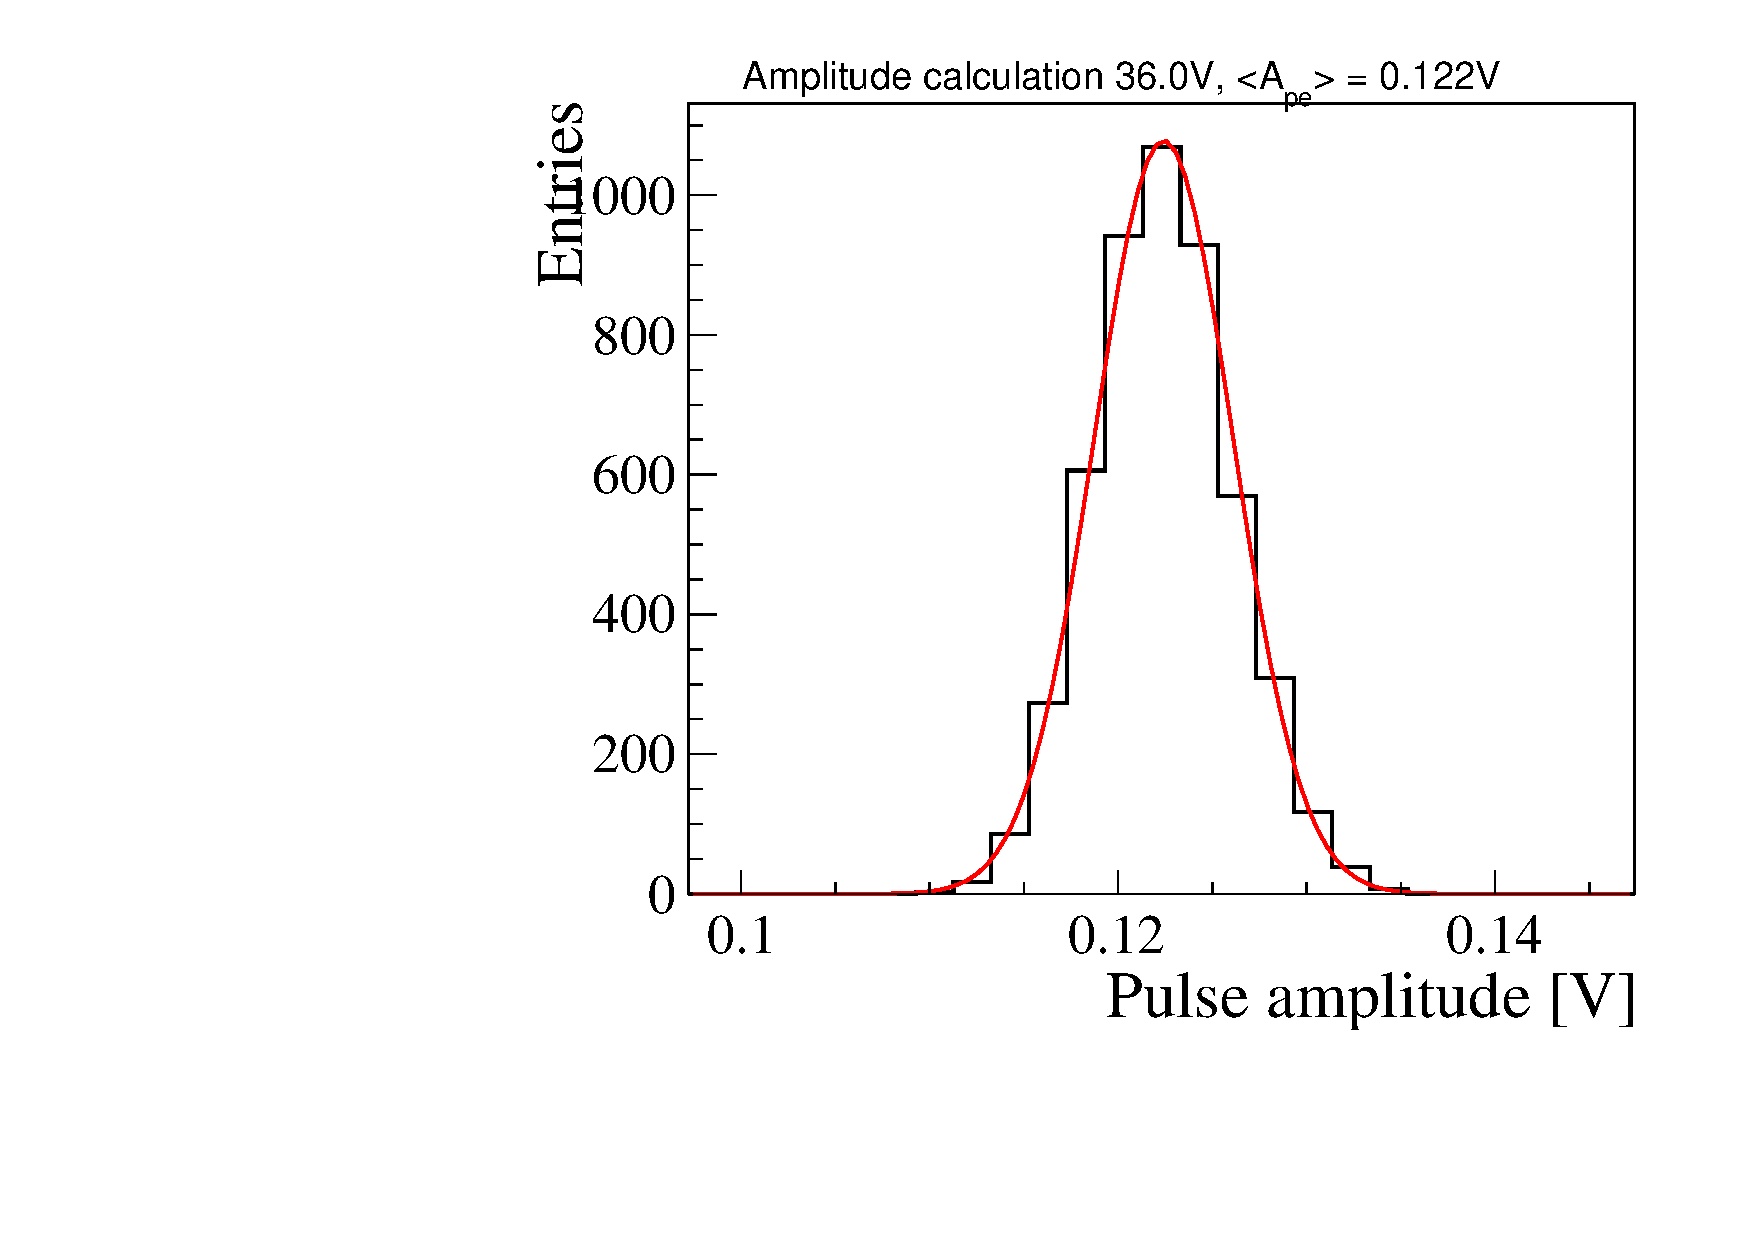
\includegraphics[width=\textwidth]{gfx/plots/examples/peakamp_36V_FBK31.pdf}
    \caption{}
  \end{subfigure}
  \hfill
  \begin{subfigure}{0.48\textwidth}
    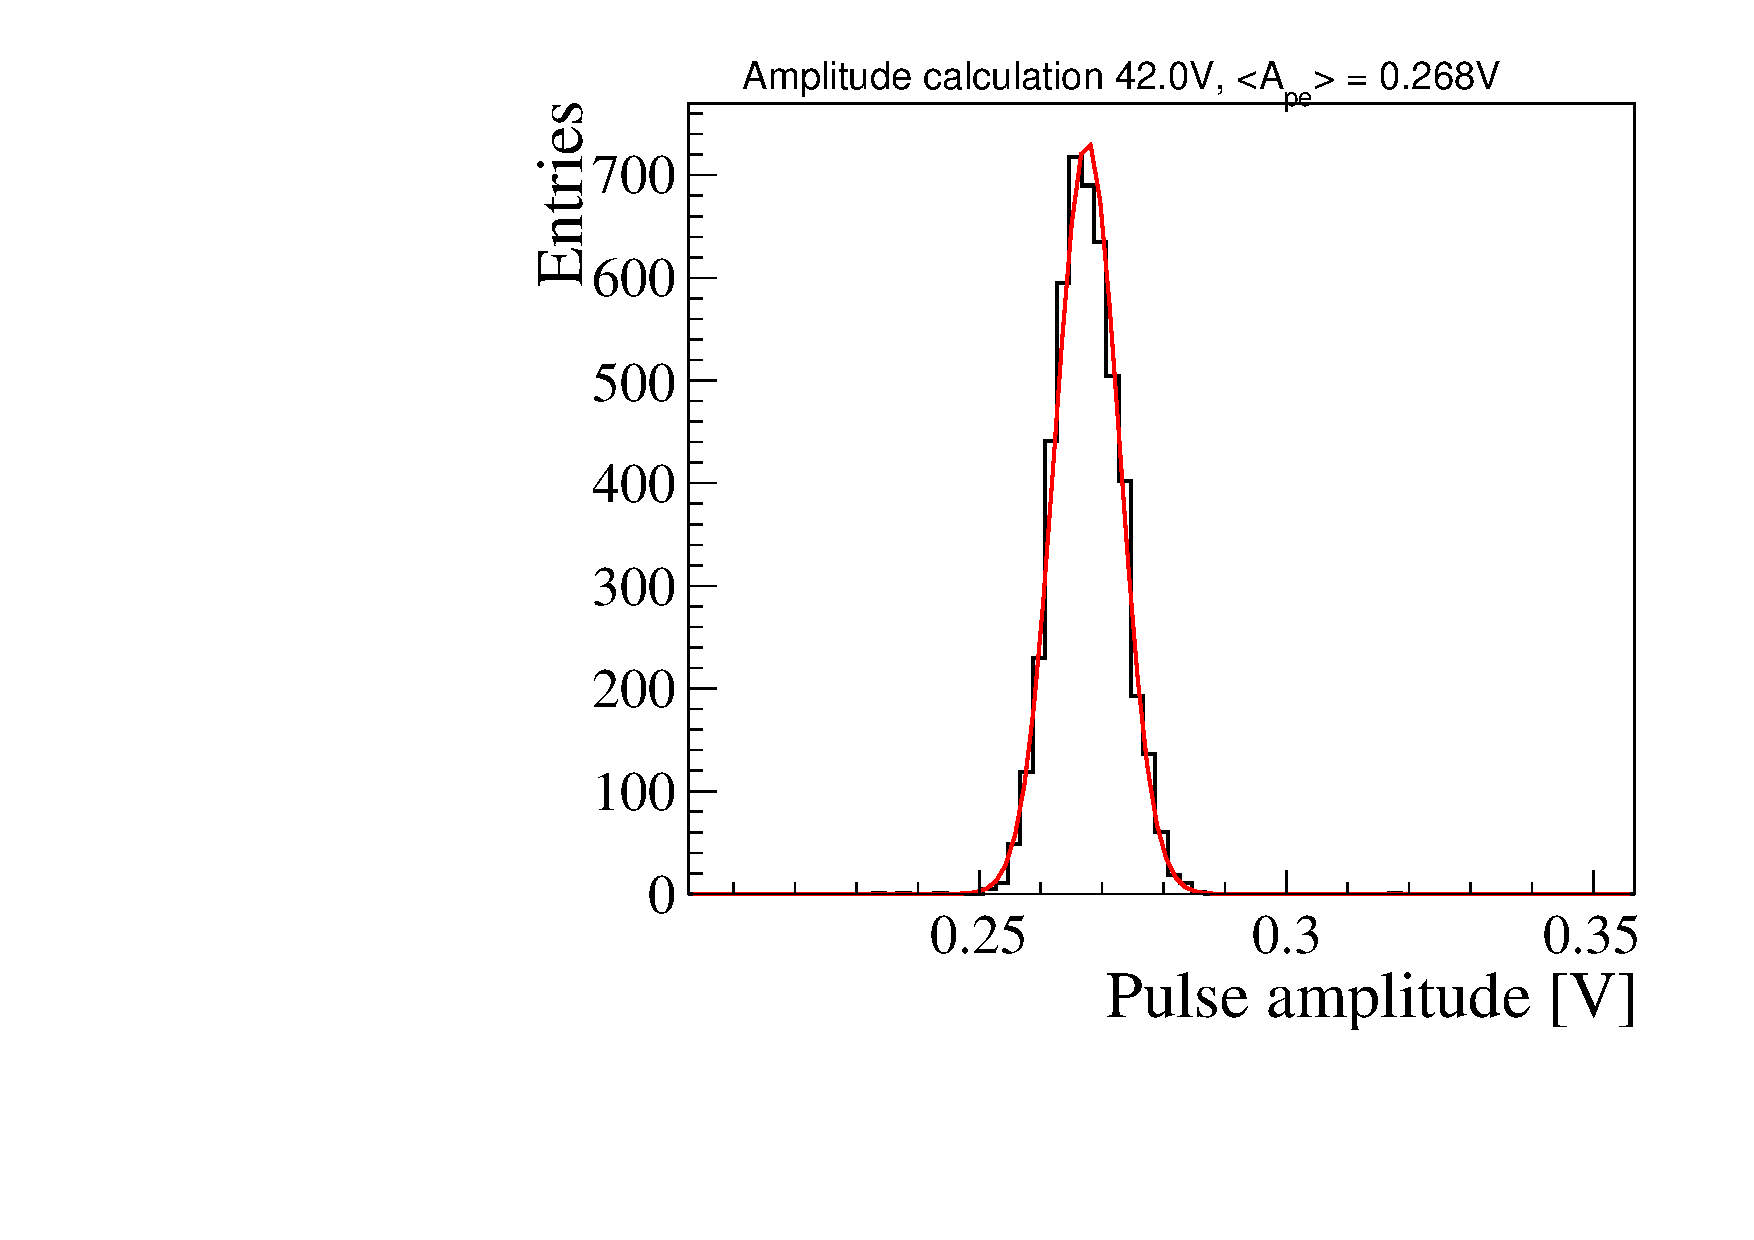
\includegraphics[width=\textwidth]{gfx/plots/examples/peakamp_42V_FBK31.pdf}
    \caption{}
  \end{subfigure}
  
  \caption{Mean peak amplitude for the SiPM FBK \SI{31}{\micro m}, channel $22$ at $5$V (a) and $11$V (b) overvoltage.}
  \label{fig:mean pulse amplitude}
\end{figure}
 


\subsection{Noise classification}
\label{ch:Experimental methods:Noise identification}
As introduced above, the waveforms are recorded by the oscilloscope and then analysed in the software. For these measurement, the temperature is fixed at \SI{25.0}{\celsius} and $5000$ waveforms are stored for each overvoltage values.

The waveform analysis software for the correlated noise is included in the determination of the breakdown voltage. To distinguish the different noises, thresholds on the time and amplitude of the waveforms need to be given as inputs. These thresholds are dependant on the SiPM pulse shape and are adapted by analysing the waveforms. This depends on the detector's features such as the value of $R_Q$ or the pixel size, etc and leads to different pulse shapes. On Fig \ref{fig:clean waveform comparison}, the difference is the pulse shape of a $1$ \ac{PE} clean signal is clearly visible. On the FBK, a plateau is present whereas on the H2017, the pulse goes to the baseline way much faster. 
\begin{figure}[htbp]
  \centering

  \begin{subfigure}{0.48\textwidth}
    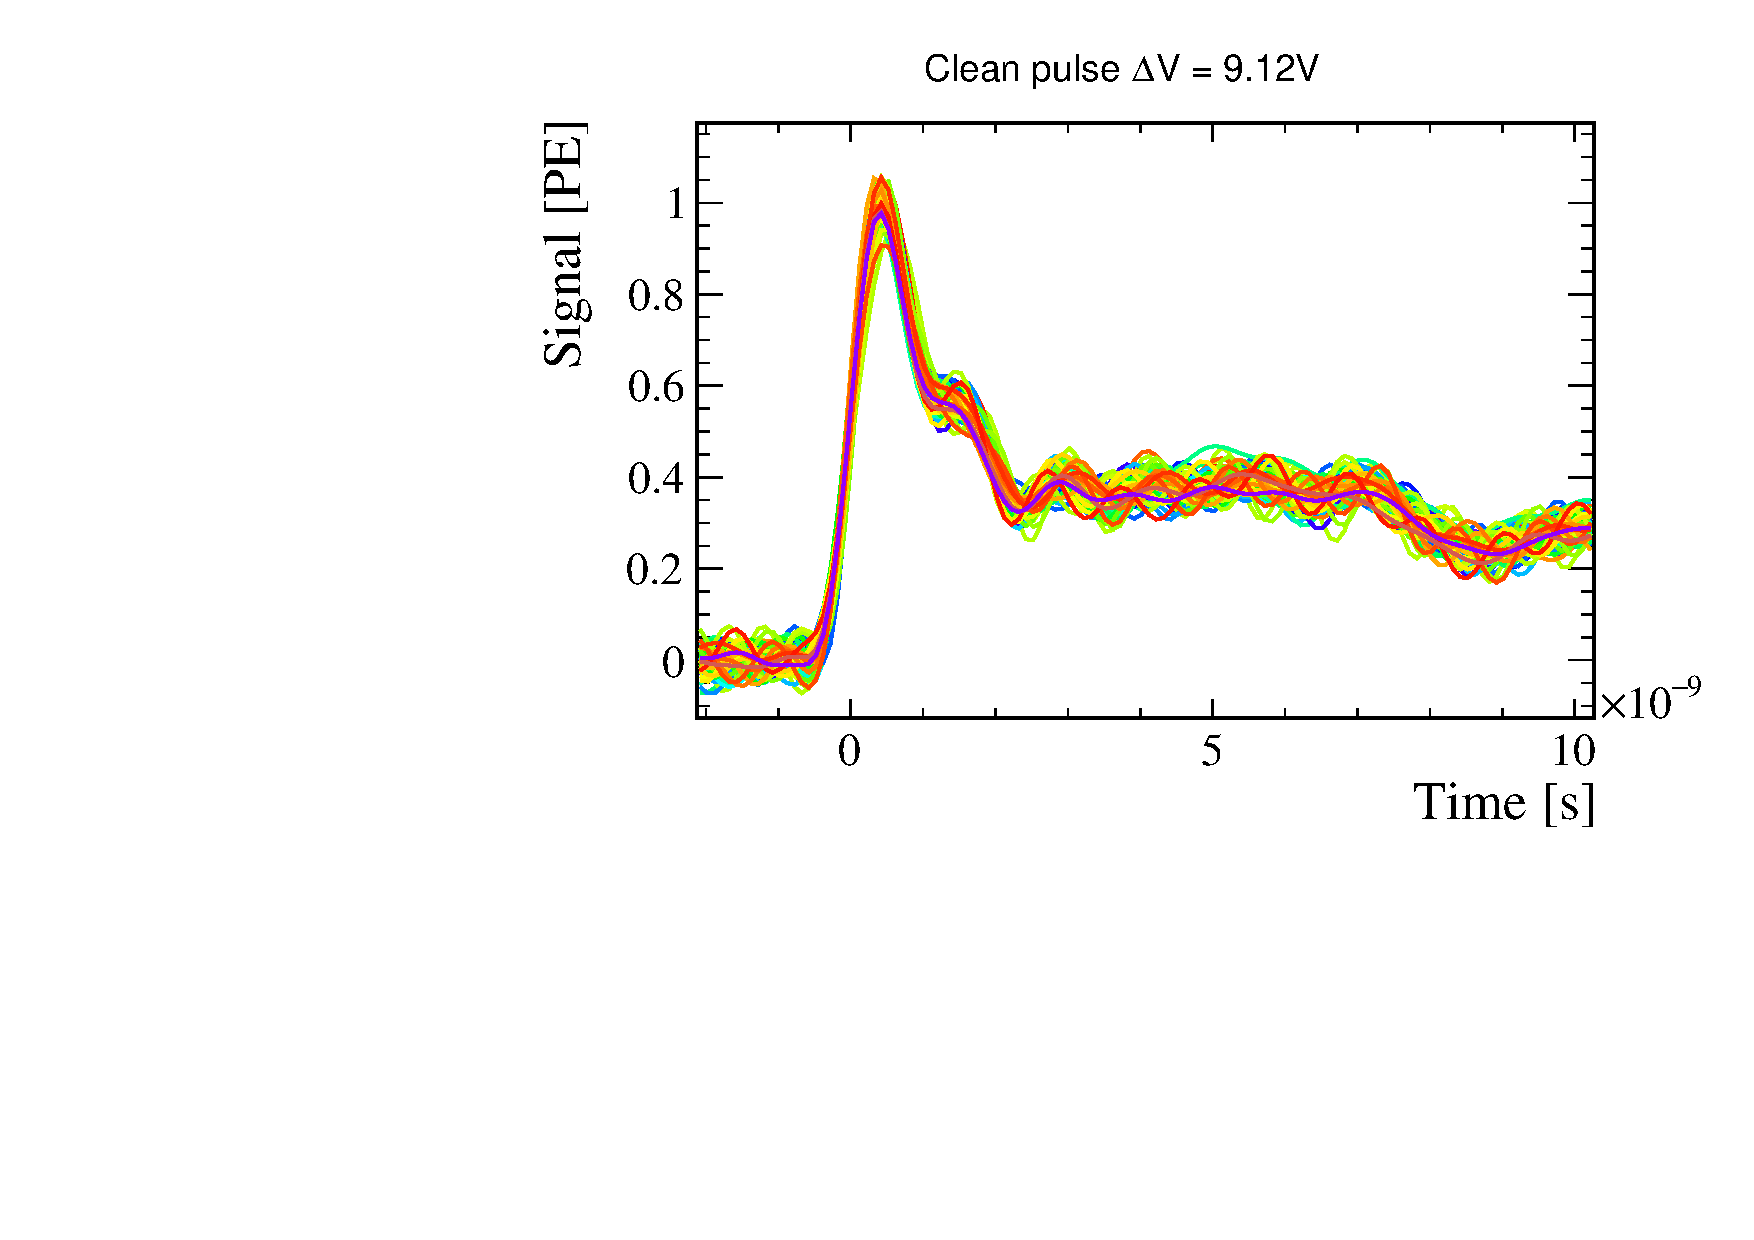
\includegraphics[width=\textwidth]{gfx/plots/WA/31/clean_10ns.pdf}
    \caption{}
    \label{fig:31/clean_10ns}
  \end{subfigure}
  \hfill
  \begin{subfigure}{0.48\textwidth}
    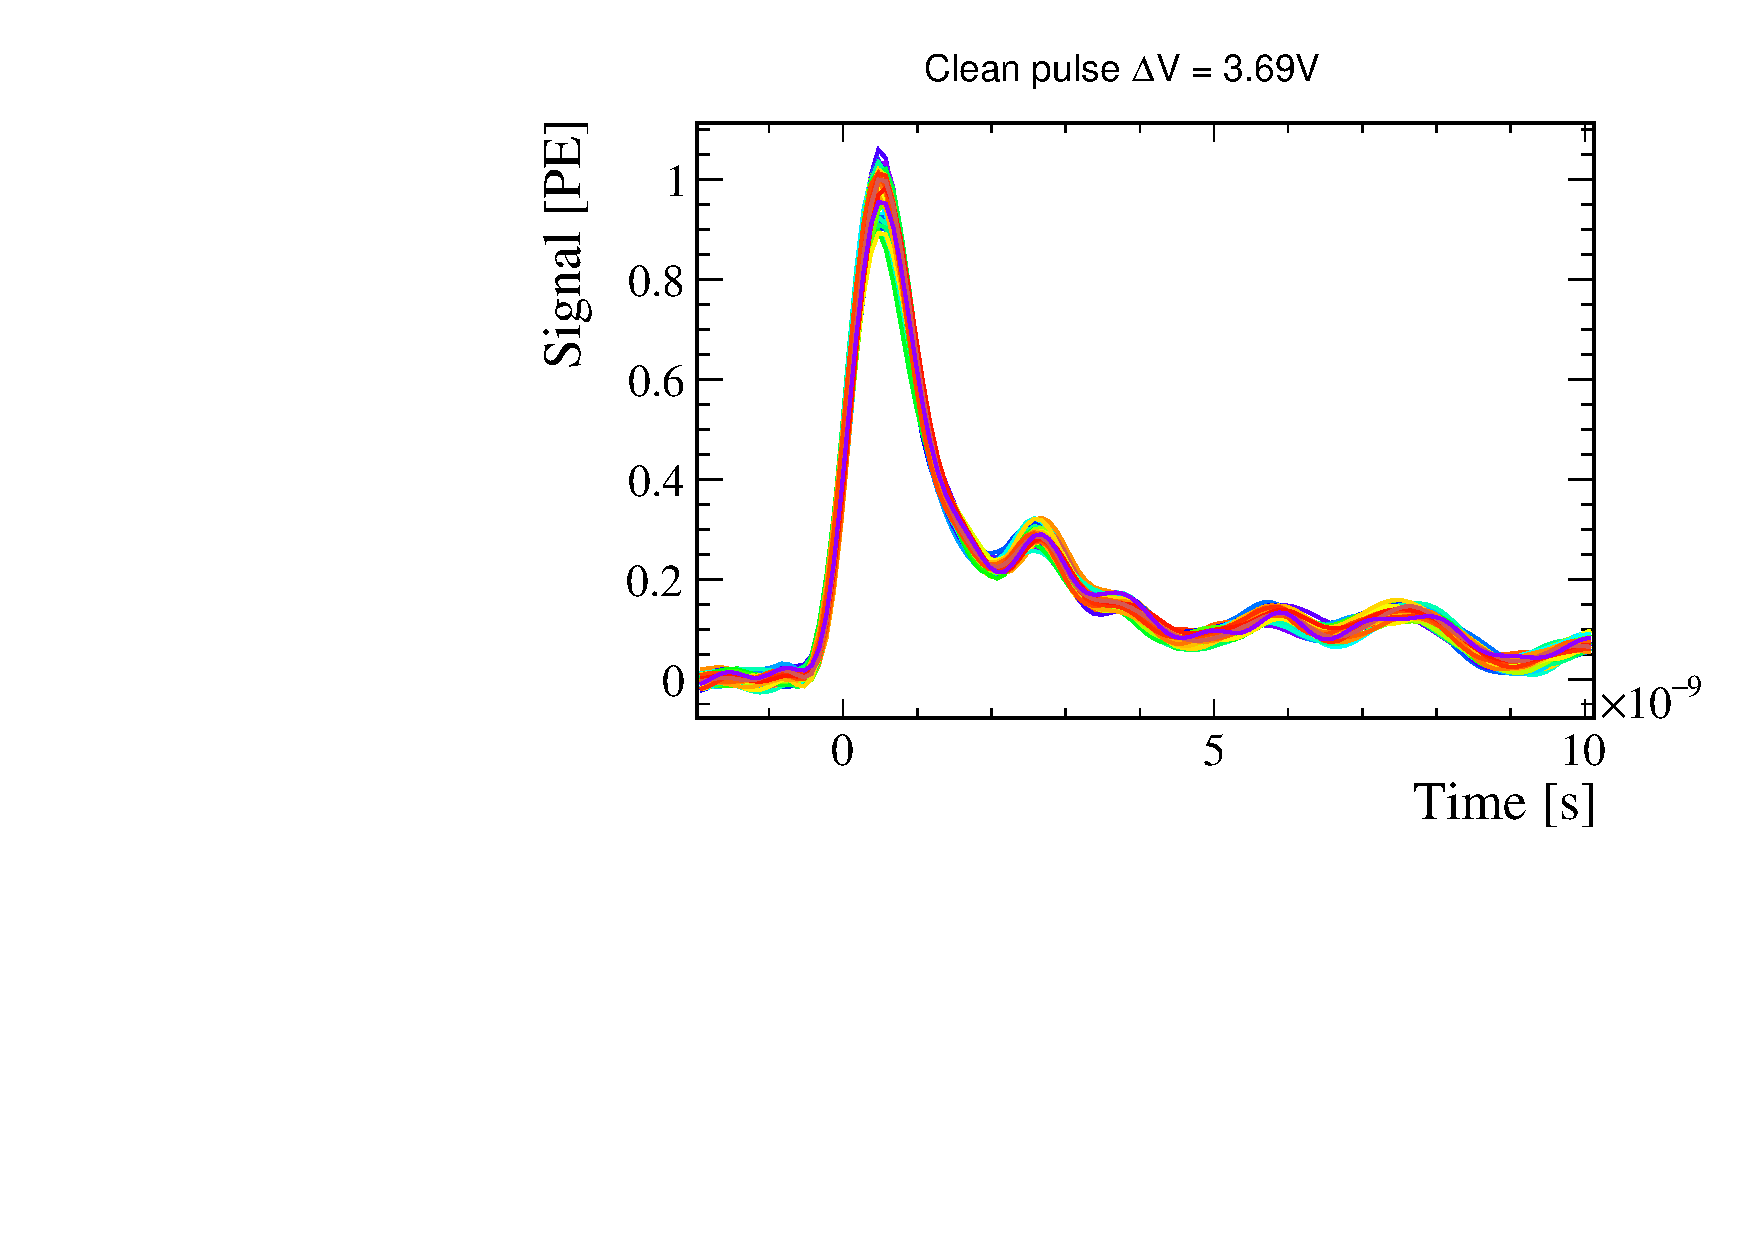
\includegraphics[width=\textwidth]{gfx/plots/WA/H2017/clean_10ns.pdf}
    \caption{}
    \label{fig:H2017/clean_10ns}
  \end{subfigure}
  \caption{FBK \SI{31}{\micro m} detector  and Hamamatsu H2017  clean waveform comparison.}
  \label{fig:clean waveform comparison}
\end{figure}

Fig. \ref{fig: mix waveforms and thresholds} shows a plot of the different waveforms for a fixed overvoltage. One can see the classification of the different correlated noises for the FBK \SI{31}{\micro m} detector. 
The results of the noise classification are presented in section \ref{ch:Results:Noise Classification}.

\begin{figure}[htbp]
  \centering
    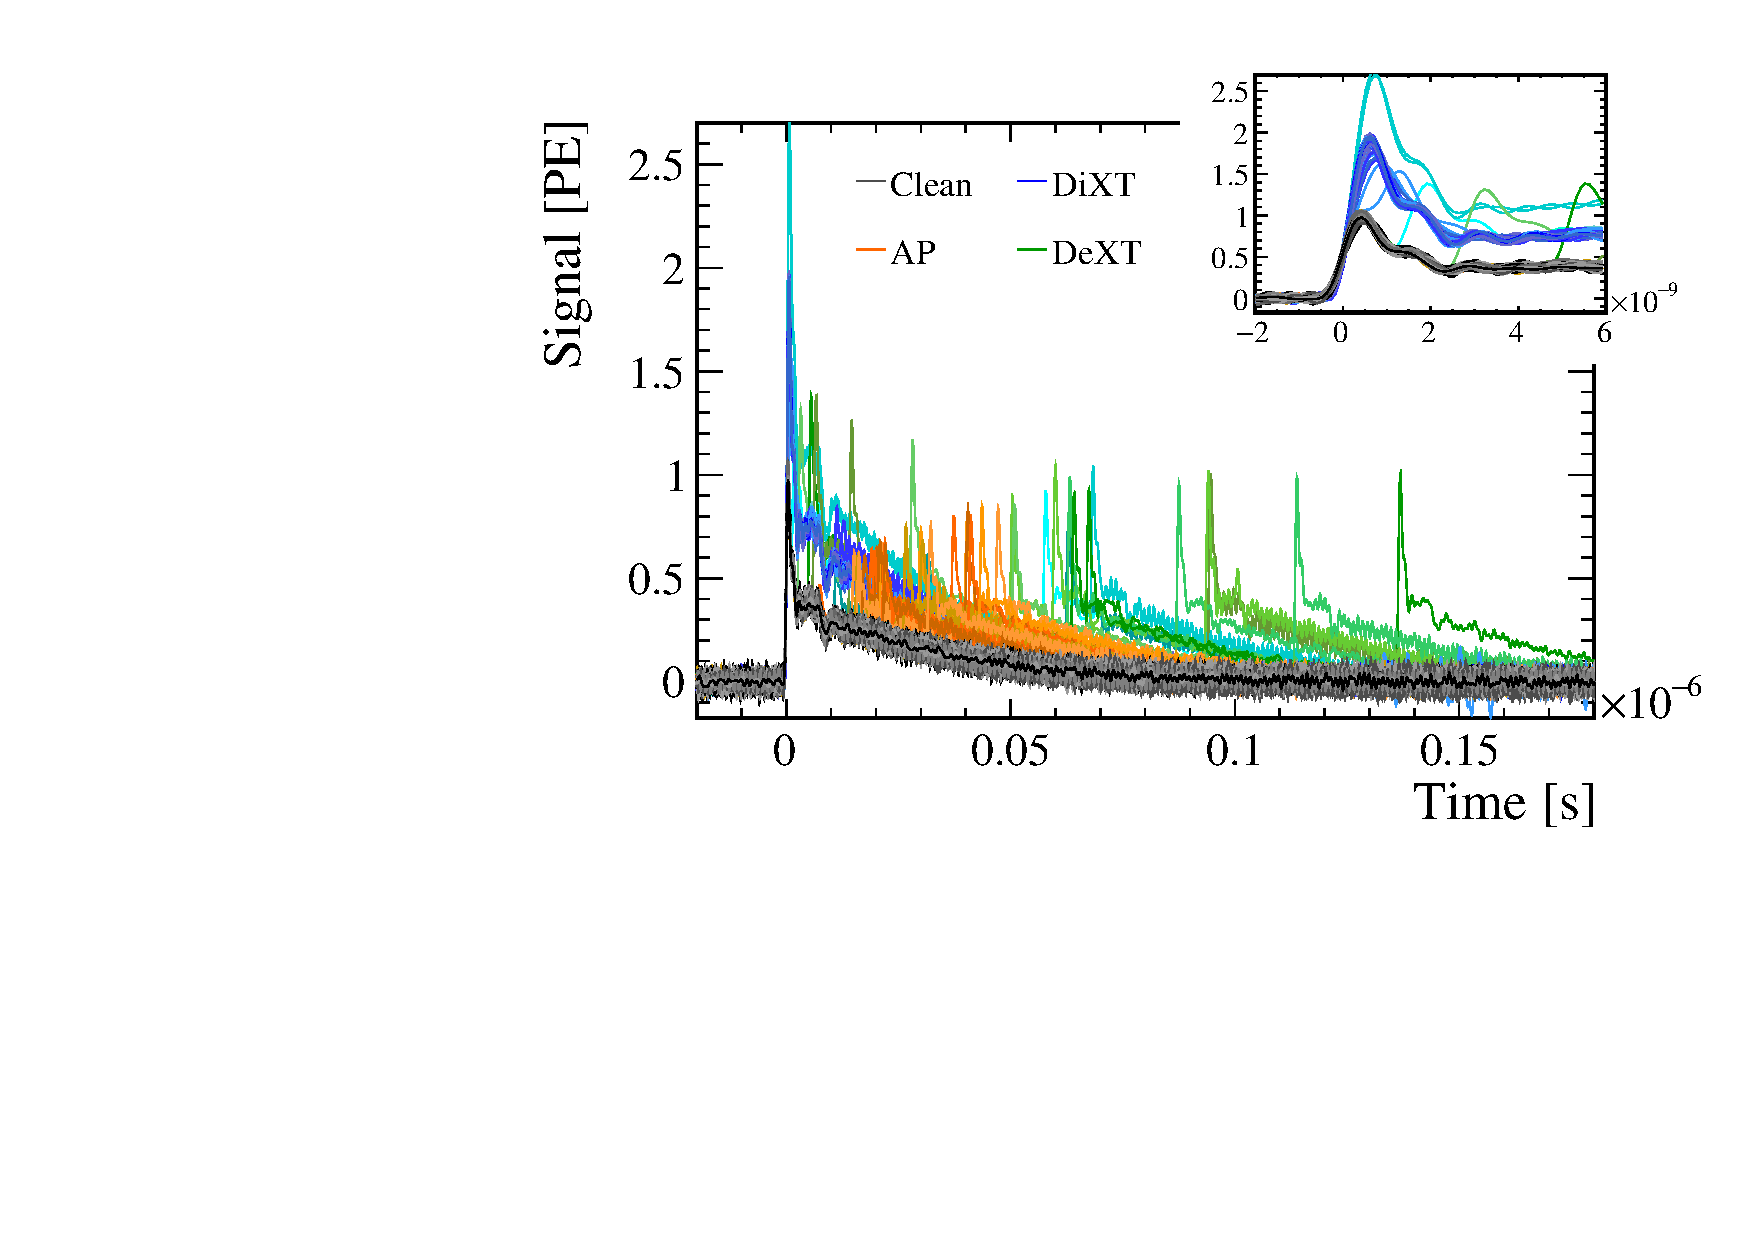
\includegraphics[width=\textwidth]{gfx/plots/WA/31/mix.pdf}
    \caption{After the analysis, different correlated noises waveforms classified (for FBK \SI{31}{\micro m} detector).}
     \label{fig: mix waveforms and thresholds}
\end{figure}


% =========== WA =========== %

% ========== PDE ==========  %



% alternative organisation



\subsection{Quenching resistor} 
\label{ch:experiement methods:WA:Rq WA}
The quenching resistor can be obtained from the waveform analysis by measuring the time constant $\tau_{long}$, which represents the slow component of the pulse shape. It is obtained by fitting the clean pulse of $1$PE as Fig. \ref{fig:taulong fit} shows. The average clean waveforms are displayed in log scale and a linear fit is applied to get the $\tau_{long}$ value. 
\begin{figure}[hbtp]
    \centering
  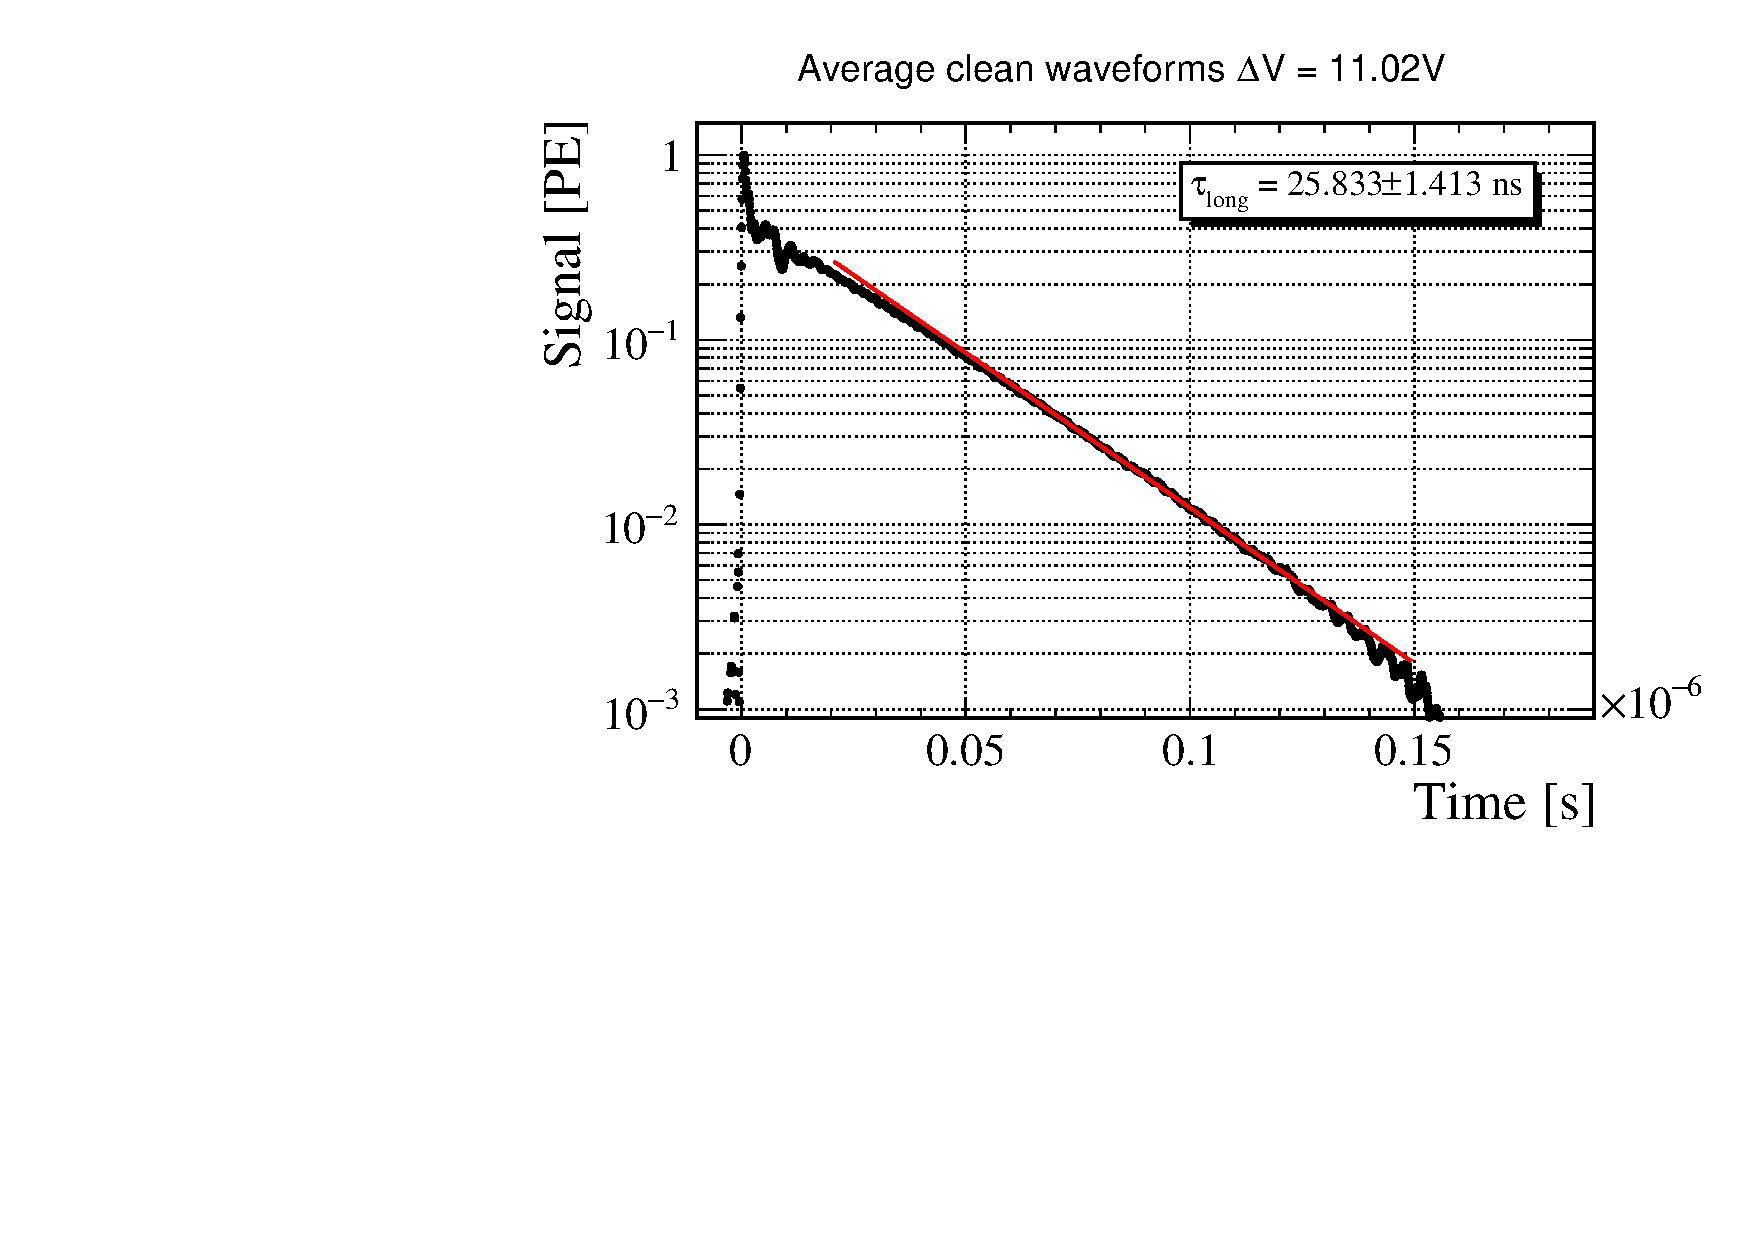
\includegraphics[width=0.7\textwidth]{gfx/plots/WA/31/taulong.pdf}
    \caption{$\tau_{long}$ determination for one overvoltage. FBK \SI{31}{\micro m}, channel $36$.}
    \label{fig:taulong fit}
\end{figure}
By knowing the average value of $\tau_{long}$ for a given detector and the diode capacitance $C_d$, one can compute $R_Q$ (Eq. \eqref{eq:Rq tau long}). $C_d$ is given by the gain measurement (Eq. \eqref{eq:Cd with gain }). The gain values are obtained as described in \ref{ch:experiement methods:Gain & PDE:gain}. 
\begin{equation*}
  \begin{minipage}[t]{0.48\linewidth}
    \begin{equation}
      \label{eq:Rq tau long}
      R_Q = \frac{\tau_{long}}{ C_d }
    \end{equation}
  \end{minipage}
  \hfill
  \begin{minipage}[t]{0.48\linewidth}
    \begin{equation}
      \label{eq:Cd with gain }
      C_d = \frac{G\cdot e}{\Delta V}
    \end{equation}
  \end{minipage}
\end{equation*}
The results are presented in section \ref{ch:Results:Rq}.
%\textbf{for each sections!!}
% =========== WA =========== %

\section{Gain and Photo-Detection Efficiency}
\label{section:Gain and Photo-Detection Efficiency}
This section is dedicated to the presentation of the setup and methods concerning Gain and Photo-Detection Efficiency.
\subsection{Setup}
\label{ch:Experimental methods:Gain and PDE:setup}
\begin{figure}[hbtp]
    \centering
    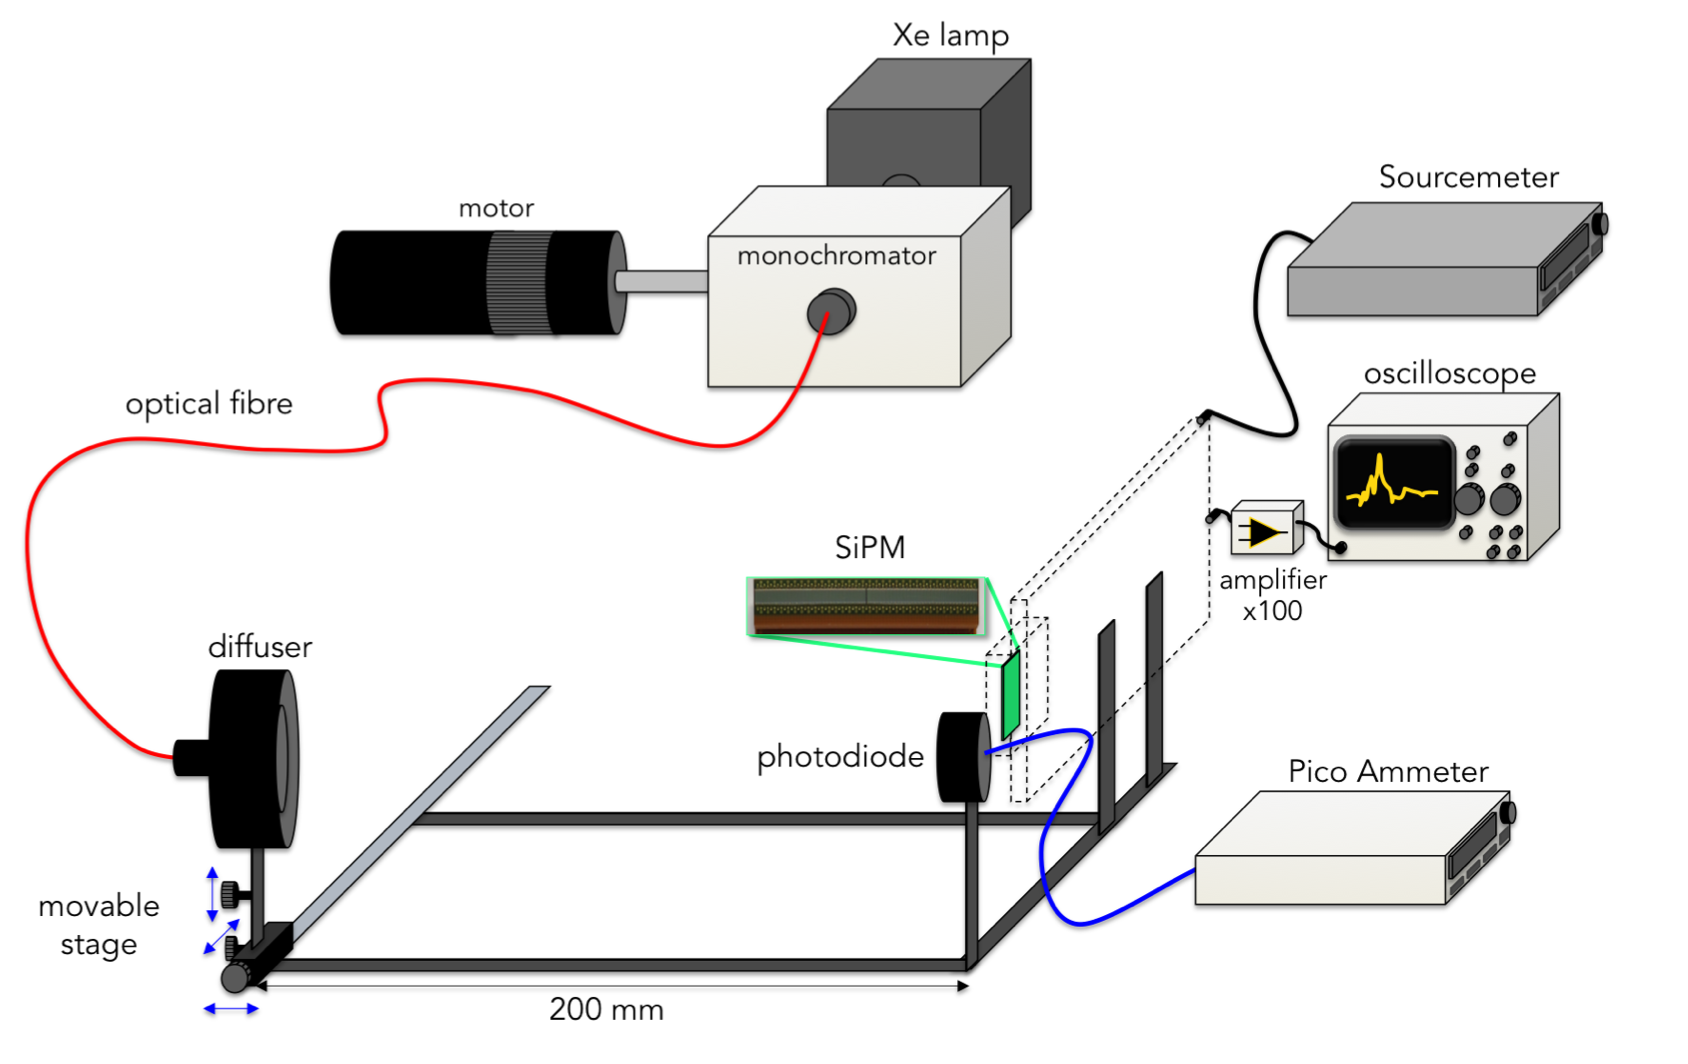
\includegraphics[width=\textwidth]{gfx/schemes/PDEsetupsketch.png}
    \caption{Scheme of the PDE setup \cite{Girard2018CharacterisationDistributions}.}
    \label{fig:PDE setup sketch}
\end{figure} 

A picture of the setup is shown in Fig. \ref{fig:PDE setup pic} and a scheme in Fig. \ref{fig:PDE setup sketch}. The light source is a Xe lamp that passes trough a monochromator\footnote{H10-UV Yvon Jobin} allowing to select a narrow wavelength interval ($\pm 1$nm). The monochromatic light now goes through a diffuser via an optical fibre. The diffused light is projected on the SiPM and a PIN diode of \SI{10.3}{mm} diameter is used for calibration\footnote{The diffuser has changed compared to \cite{Girard2018CharacterisationDistributions}.}. It is sensible from \SI{160}{\nano m} to \SI{900}{\nano m} and its photo-current is measured with a pico ammeter\footnote{KEITHLEY 6485 PICOAMMETER}. 


Three different measurements are taken to acquire the needed data for the gain and PDE. First, the diode calibration data consists in measuring the current produced by the PIN diode for each wavelength $\lambda$.  As Eq. \eqref{eq:Frequency PDE} and Eq. \eqref{eq:Current PDE} show, calibration data from the PIN Diode is crucial (dependency of $I_{PD}(\lambda)$), because this calibration allows to know how many photons are projected on the SiPM surface $A_{SiPM}$. The calibration data should be taken regularly, with a constant temperature during the measurement, fixed at $T_{meas} = 25.0 ^{\circ}$C.
\\
After the calibration comes the acquisition of the dark count rate and dark current of the studied detector. As in \ref{ch:Experimental methods:Noise identification}, a black cloth is wrapped around the detector so that only noise is present. The oscilloscope counts the number of peaks higher than $0.6$PE for a time window of \SI{100}{\micro s} for every $\Delta V$. In the mean time, the current produced by the SiPM is recorded for every $\Delta V$ too.
\\
The third and last measurement is the "light" data. The SiPM is placed in front of the diffuser and the measurement are the same as in the dark but now for all $\lambda$ in addition to every $\Delta V$.
\\
As mentioned before, the PIN Diode and the SiPM are mounted on motorized rails. The light beam should be perfectly aligned with the measured device. One can plot the current of the SiPM and PIN Diode as a function of the horizontal position, shown in Fig. \ref{fig:light alignment positions}
\begin{figure}[http]
    \centering    
    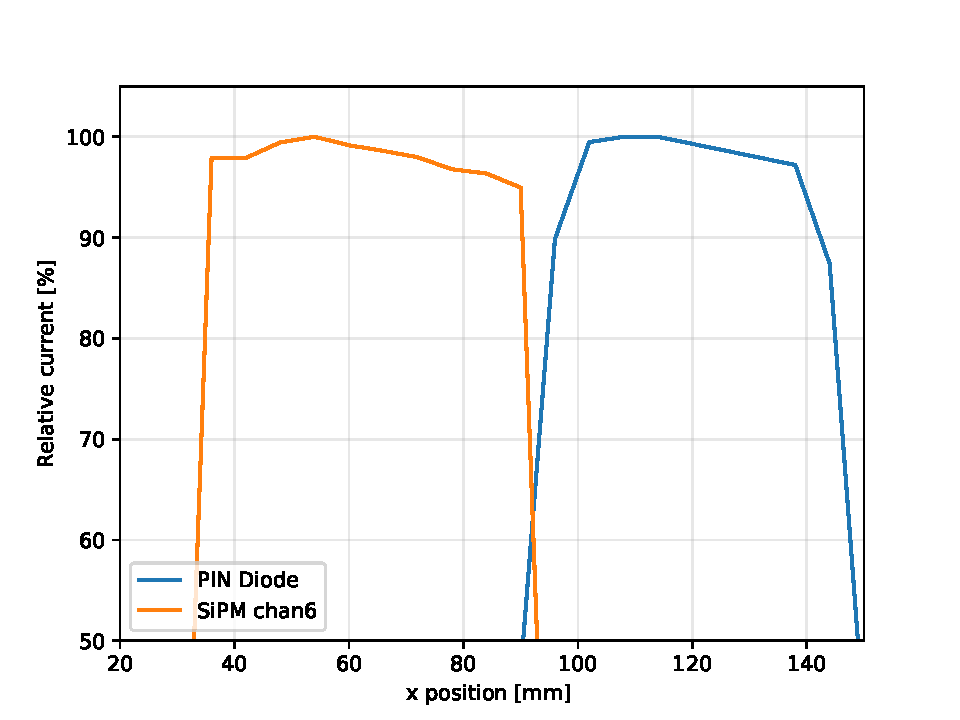
\includegraphics[width=0.8\textwidth]{gfx/plots/positions.pdf}
    \caption{Measured relative photo-current of the PIN diode and the SiPM as a function of the horizontal position. }
    \label{fig:light alignment positions}
\end{figure}
Hence, from this plot the position for the perfect alignment can be found for the channel $6$  which is $60 $ mm and the PIN Diode $120 $ mm. The same can be obtained for any channel as Eq. \eqref{eq:light alignement} shows (position in mm):

\begin{equation}
    x(channel) = 60 - channel\cdot250\cdot 10^{-3}
    \label{eq:light alignement}
\end{equation}

%\textbf{Better homogeneity plot}
%\textbf{Add a H. plot for the H2017}


\subsection{Gain}
\label{ch:experiement methods:Gain & PDE:gain}
The gain is measured with the light data and computed as in Eq. \eqref{eq: gain computation}. For each $\Delta V$ and $\lambda$, the photo-current $I_{light}(\Delta V, \lambda)$ is measured and corrected with the proportion of DiXT. $P_{DiXT}(\Delta V)$ is the probability of direct cross talk measured in the waveform analysis (see \ref{section:waveform analysis}). This corrected value is divided by $F_{light}$ which is the rate of peaks over the time interval selected by the oscilloscope (\SI{100}{\micro s}). The ratio: $$\frac{I_{light}(\Delta V, \lambda)\cdot(1-P_{DiXT}(\Delta V))}{F_{light}}$$ is then the total charge generated. To finally get the gain, we divide the total charge by the elementary charge $e$. No significant variations are observed with $\lambda$ so we take the average over $\lambda$: 
\begin{equation}
    G_{light}(\Delta V) = \frac{I_{light}(\Delta V)\cdot(1-P_{DiXT}(\Delta V))}{ F_{light}(\Delta V)\cdot e}
    \label{eq:gaincomputation}
\end{equation}

\paragraph{uncertainties.} The statistical uncertainties are again negligible since the they represents $0.1\%$. By measuring the several times the gain, the systematics uncertainties are estimated at $2\%$. Results are presented in \ref{ch:Results:Gain}.


\subsection{Photo-Detection Efficiency} 
\label{ch:experiement methods:Gain & PDE:PDE}

There are two ways of measuring the PDE:

\paragraph{Current method:} The current method uses the current recorded from the light and dark data explained in \ref{ch:Experimental methods:Gain and PDE:setup}. 
It exploits the measurement on the gain value $G_{light}(\Delta V)$, measured as described in section \ref{ch:experiement methods:Gain & PDE:gain}. 
Where $I_{PD}(\lambda)$ is the current produced by the PIN diode in the calibration data. $A_{PD}$ and $A_{SiPM}$ are the areas of the PIN diode and the SiPM channel respectively. 
The correction on the current takes into account the primary and secondary noises. The measured current $I^*$ corresponds to Eq. \eqref{eq: correction measured current}
\begin{equation}
    I^{*}= I_{light}\cdot(1+ r_{current})
    \label{eq: correction measured current}
\end{equation}
\begin{equation*}
    r_{current } =P_{DeXT} + P_{DiXT}+ w_{AP}\cdot P_{AP} + w_{ho}\cdot P_{ho}
    \label{eq: correction r current}  
\end{equation*}
Where $ w_{AP}$ \& $w_{ho}$ are the mean amplitude of the after-pulse and higher order peaks respectively.
At first approximation (since $r_{current} \ll 1$), taking into account the measured dark current $I_{DCR}$, the current is then corrected as Eq.\eqref{eq:correction I}:
\begin{equation}
    I_{light} = (I^{*}-I_{DCR})\cdot(1-r_{current})
    \label{eq:correction I}
\end{equation}
These values of amplitude and probabilities are measured in \ref{ch:Experimental methods:Noise identification}.

The final equation for the current PDE is then Eq. \eqref{eq:Current PDE}:
\begin{equation}
    \texttt{PDE}_{curr}(\Delta V, \lambda) = \frac{\left(I^{*}(\Delta V, \lambda)-I_{DCR}(\Delta V)\right)\cdot(1-r_{current}(\Delta V))}{I_{PD}(\lambda)\cdot G_{light, mean}(\Delta V)}\cdot \frac{A_{PD}}{A_{SiPM}} 
    \label{eq:Current PDE}
\end{equation}


\paragraph{Rate method:} For each wavelength $\lambda$, and each over voltage $\Delta V$, the number of peaks are counted by the oscilloscope on a given time window of $\Delta t =$ \SI{100}{\micro s}. This allows to not correct for DiXT since only peaks above a $0.6$PE thresholds are counted and not their amplitude. The rate is obtained by counting the peak on a given time window. The rate in the dark is called $F_{DCR}$ while the rate in the SiPM illuminated is called $F_{light}$. 
As for the current method, the measured rate $F^*$ do not correspond to the rate produced $F_{light}$ only by light detection. It needs to be corrected as in Eq. \eqref{eq:rate correction}:
\begin{equation}
    F^{*} = F_{light}\cdot(1+ r_{rate})
    \label{eq:rate correction}
\end{equation}
\begin{equation*}
    r_{rate} = P_{DeXT} + P_{AP}^{0.6} +P_{ho}^{rate}
    \label{eq: correction r current}  
\end{equation*}
Therefore, the rate in the light corrected is given by Eq. \eqref{eq:rate light}:
\begin{equation}
    F_{light}= (F^* - F_{DCR})\cdot(1-r_{rate})
    \label{eq:rate light}
\end{equation}
The equation to calculate the PDE using this method is: Eq. \eqref{eq:Frequency PDE}. 
\begin{equation}
    \texttt{PDE}_{freq}(\Delta V, \lambda) = \frac{\left(F^{*}(\Delta V, \lambda)-F_{DCR}(\Delta V)\right)\cdot(1-r_{rate}(\Delta V))}{e \cdot I_{PD}(\lambda)}\cdot \frac{A_{PD}}{A_{SiPM}}
    \label{eq:Frequency PDE}
\end{equation}
The rate method does not require the gain and then the uncertainties are reduced. For noise measurements with a large amount higher order peaks, the PDE may over correct as overvoltage increases resulting in an underestimation of PDE. A fine tuning of the thresholds in the waveform analysis needs to be done to get accurate PDE results. 
Results are presented in \ref{ch:Results:PDE}.
